\documentclass[
  10pt,
  aspectratio=169,
  utf8,
  xcolor={dvipsnames}
]{beamer}

\usetheme[
  progressbar=foot,
  sectionpage=progressbar,
  subsectionpage=progressbar,
  numbering=fraction
]{metropolis}
\usefonttheme{metropolis}
\usecolortheme{spruce}
\setbeamercolor{progress bar}{fg=MidnightBlue, bg=LightSteelBlue}
\setbeamercolor{title}{fg=MidnightBlue}
\setbeamercolor{frame title}{fg=MidnightBlue}
\setbeamercolor{structure}{fg=MidnightBlue}

\usepackage{booktabs}
\usepackage{graphicx}
\usepackage{tikz}
\usetikzlibrary{shapes, arrows, positioning, fit, backgrounds}
\usepackage{amsmath}
\usepackage{amssymb}
\usepackage{fontspec}
\usepackage{caption}
\captionsetup[figure]{labelformat=empty}
\captionsetup[table]{labelformat=empty}

\title{\textbf{The Cox Proportional Hazards Model and Hazard Ratios}}
\subtitle{Quantitative and Modeling - SDS6210 Informatics for Health}
\author{\textbf{Cavin Otieno}}
\institute{Department of Public Health\\University}
\date{\today}

\begin{document}

% Group Members Frame
{
\setbeamertemplate{footline}{}
\begin{frame}
\titlepage
\end{frame}
}

\begin{frame}{Group 5 Members}
\begin{center}
\begin{tabular}{ll}
\toprule
\textbf{Student ID} & \textbf{Student Name} \\
\midrule
SDS6/46982/2024 & Cavin Otieno \\
SDS6/47543/2024 & Laura Nabalayo Kundu \\
SDS6/47659/2024 & John Andrew \\
\bottomrule
\end{tabular}
\end{center}
\end{frame}

\begin{frame}{Outline}
\tableofcontents
\end{frame}

% ============================================================================
% SECTION 1: FUNDAMENTALS OF SURVIVAL ANALYSIS
% ============================================================================

\section{Fundamentals of Survival Analysis}

\subsection{Survival Time and Censoring}

\begin{frame}{Survival Data: Time-to-Event Analysis}
Survival analysis studies the time until the occurrence of a specific event:

\begin{block}{Definition of Survival Time}
Let $T$ denote the survival time, defined as the time from a defined origin (e.g., diagnosis, treatment initiation) to the occurrence of a specified event (e.g., death, disease recurrence, recovery).
\end{block}

\begin{center}
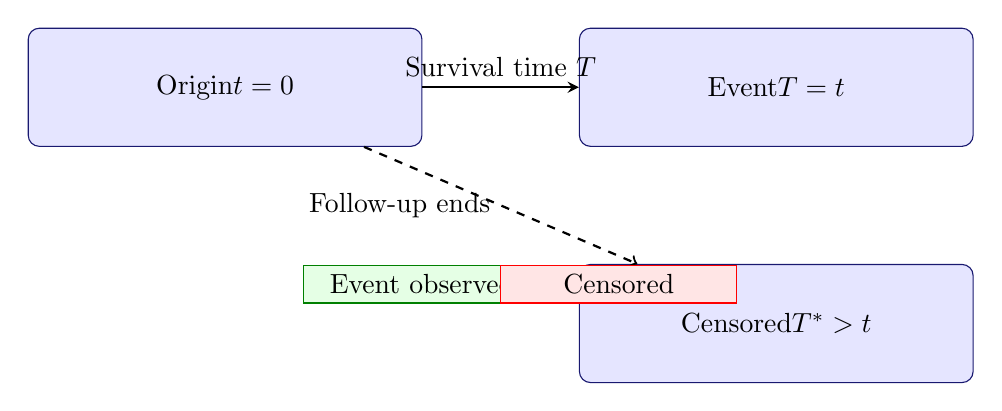
\begin{tikzpicture}[node distance=2cm]
\tikzstyle{block} = [rectangle, rounded corners, minimum width=5cm, minimum height=1.5cm, text centered, draw=MidnightBlue, fill=blue!10]

\node (origin) [block] {Origin\\$t=0$};
\node (event) [block, right of=origin, xshift=5cm] {Event\\$T=t$};
\node (censored) [block, below of=event, yshift=-1cm] {Censored\\$T^* > t$};

\draw[->, thick, >=stealth] (origin) -- (event) node[midway, above] {Survival time $T$};
\draw[->, thick, dashed] (origin) -- (censored) node[midway, left] {Follow-up ends};

\node at (2.5, -2.5) [rectangle, draw=Green, fill=green!10, minimum width=3cm] {Event observed};
\node at (5, -2.5) [rectangle, draw=Red, fill=red!10, minimum width=3cm] {Censored};
\end{tikzpicture}
\end{center}
\end{frame}

\begin{frame}{Censoring: The Central Challenge}
In survival analysis, complete event times are often not observed:

\begin{block}{Types of Censoring}
\begin{columns}
\begin{column}{0.5\textwidth}
\begin{block}{Right Censoring}
The event has not occurred by the end of the study period. We know $T > c$ where $c$ is the censoring time.
\end{block}
\end{column}
\begin{column}{0.5\textwidth}
\begin{block}{Left Censoring}
The event occurred before the study began. We know $T < c$.
\end{block}
\end{column}
\end{columns}
\end{block}

\begin{block}{Data Representation}
For each subject $i = 1, \ldots, n$:
\begin{itemize}
\item $t_i$: The observed time (minimum of survival time and censoring time)
\item $\delta_i$: The event indicator
\begin{equation*}
\delta_i = \begin{cases} 1 & \text{if } t_i = T_i \text{ (event observed)} \\ 0 & \text{if } t_i = C_i \text{ (censored)} \end{cases}
\end{equation*}
\end{itemize}
\end{block}
\end{frame}

\begin{frame}{Implications of Censoring for Analysis}
Censoring is non-informative if the probability of being censored is independent of the event:

\begin{block}{Assumptions About Censoring}
\begin{itemize}
\item \textbf{Non-informative censoring}: The censoring mechanism is independent of the event time
\item \textbf{Random censoring}: Censoring times are independent of survival times
\end{itemize}
\end{block}

\begin{center}
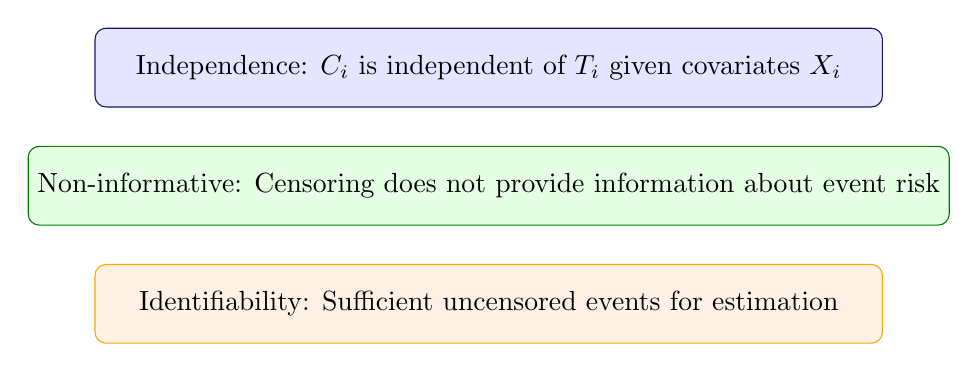
\begin{tikzpicture}[node distance=1.5cm]
\tikzstyle{assumption} = [rectangle, rounded corners, minimum width=10cm, minimum height=1cm, text centered]

\node (A1) [assumption, draw=MidnightBlue, fill=blue!10] {Independence: $C_i$ is independent of $T_i$ given covariates $X_i$};
\node (A2) [assumption, below of=A1, draw=Green, fill=green!10] {Non-informative: Censoring does not provide information about event risk};
\node (A3) [assumption, below of=A2, draw=Orange, fill=orange!10] {Identifiability: Sufficient uncensored events for estimation};
\end{tikzpicture}
\end{center}
\end{frame}

\subsection{The Hazard and Survival Functions}

\begin{frame}{The Survival Function}
The survival function gives the probability of surviving beyond time $t$:

\begin{definition}[Survival Function]
$$S(t) = P(T > t)$$
This represents the probability that the event has not occurred by time $t$.
\end{definition}

\begin{block}{Properties of $S(t)$}
\begin{itemize}
\item $S(0) = 1$ (all subjects survive at time 0)
\item $S(t)$ is non-increasing: $S(u) \leq S(t)$ for $u > t$
\item $\lim_{t \to \infty} S(t) = 0$ (the event eventually occurs)
\end{itemize}
\end{block}

\begin{center}
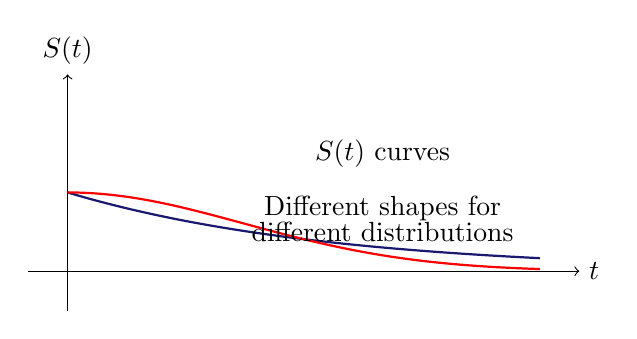
\begin{tikzpicture}[domain=0:6, smooth, samples=100]
\draw[->] (-0.5,0) -- (6.5,0) node[right] {$t$};
\draw[->] (0,-0.5) -- (0,2.5) node[above] {$S(t)$};

\draw[thick, MidnightBlue] plot (\x, {exp(-0.3*\x)});
\draw[thick, red] plot (\x, {exp(-0.1*\x*\x)});

\node at (4,1.5) {$S(t)$ curves};
\node at (4,0.8) {Different shapes for};
\node at (4,0.5) {different distributions};
\end{tikzpicture}
\end{center}
\end{frame}

\begin{frame}{The Hazard Function}
The hazard function describes the instantaneous risk of the event at time $t$, conditional on survival to that time:

\begin{definition}[Hazard Function]
$$h(t) = \lim_{\Delta t \to 0} \frac{P(t \leq T < t + \Delta t \mid T \geq t)}{\Delta t}$$
\end{definition}

\begin{block}{Interpretation}
The hazard function represents:
\begin{itemize}
\item The instantaneous event rate at time $t$ among those at risk
\item A measure of how the risk of the event changes over time
\end{itemize}
\end{block}

\begin{block}{Relationship to Survival Function}
\begin{align*}
h(t) &= -\frac{d}{dt} \log S(t) \\
S(t) &= \exp\left(-\int_0^t h(u) \, du\right)
\end{align*}
where $\int_0^t h(u) \, du$ is the cumulative hazard function $H(t)$.
\end{block}
\end{frame}

\begin{frame}{Hazard vs. Survival: Conceptual Distinction}
\begin{center}
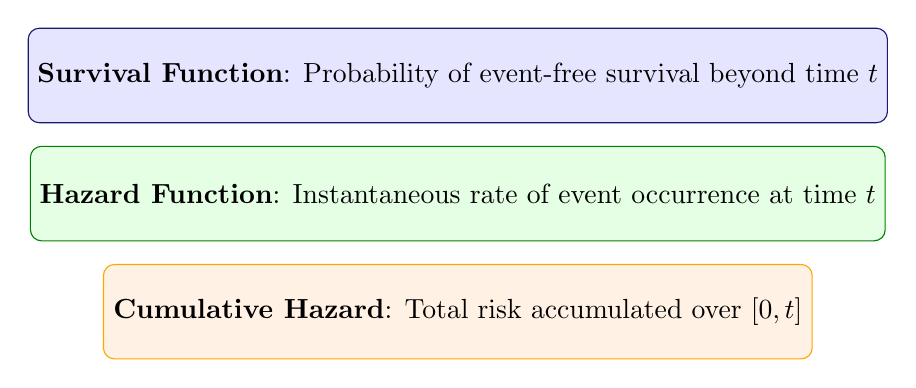
\begin{tikzpicture}[node distance=1.5cm]
\tikzstyle{comparison} = [rectangle, rounded corners, minimum width=9cm, minimum height=1.2cm, text centered]

\node (C1) [comparison, draw=MidnightBlue, fill=blue!10] {\textbf{Survival Function}: Probability of event-free survival beyond time $t$};
\node (C2) [comparison, below of=C1, draw=Green, fill=green!10] {\textbf{Hazard Function}: Instantaneous rate of event occurrence at time $t$};

\node (C3) [comparison, below of=C2, draw=Orange, fill=orange!10] {\textbf{Cumulative Hazard}: Total risk accumulated over $[0, t]$};
\end{tikzpicture}
\end{center}

\begin{block}{Example: Post-Surgical Recovery}
\begin{center}
\begin{tabular}{lll}
\toprule
Time Period & Hazard Shape & Interpretation \\
\midrule
Immediately post-op & High & Surgical complications \\
Recovery period & Decreasing & Healing over time \\
Long-term follow-up & Low/stable & Baseline risk \\
\bottomrule
\end{tabular}
\end{center}
\end{block}
\end{frame}

% ============================================================================
% SECTION 2: THE COX PROPORTIONAL HAZARDS MODEL
% ============================================================================

\section{The Cox Proportional Hazards Model}

\subsection{Model Formulation}

\begin{frame}{The Cox Model: A Regression Framework for Survival Data}
The Cox proportional hazards model extends regression to time-to-event data:

\begin{alertblock}{The Cox Model Equation}
$$h(t|X) = h_0(t) \exp\left(\beta_1 X_1 + \beta_2 X_2 + \cdots + \beta_k X_k\right)$$
\end{alertblock}

\begin{columns}
\begin{column}{0.5\textwidth}
\begin{block}{Model Components}
\begin{itemize}
\item $h(t|X)$: Hazard at time $t$ given covariates $X$
\item $h_0(t)$: Baseline hazard function
\item $X = (X_1, \ldots, X_k)$: Vector of covariates
\item $\beta = (\beta_1, \ldots, \beta_k)$: Vector of coefficients
\end{itemize}
\end{block}
\end{column}
\begin{column}{0.5\textwidth}
\begin{block}{Model Classification}
\textbf{Semi-parametric}:
\begin{itemize}
\item The baseline hazard $h_0(t)$ is non-parametric (unspecified form)
\item The covariate effects are parametric (multiplicative on hazard scale)
\end{itemize}
\end{block}
\end{column}
\end{columns}
\end{frame}

\begin{frame}{The Baseline Hazard Function}
The baseline hazard $h_0(t)$ represents the hazard for an individual with all covariates equal to zero:

\begin{block}{Properties of $h_0(t)$}
\begin{itemize}
\item Non-parametric: No distributional assumption required
\item Unknown function that can take any non-negative shape
\item Acts as a time-varying intercept in the model
\end{itemize}
\end{block}

\begin{block}{Interpretation}
If $X = 0$ (all covariates at reference levels):
$$h(0,t) = h_0(t) \cdot \exp(0) = h_0(t)$$
Thus $h_0(t)$ is the hazard for the reference individual/group.
\end{block}

\begin{block}{Advantages of Semi-Parametric Form}
\begin{center}
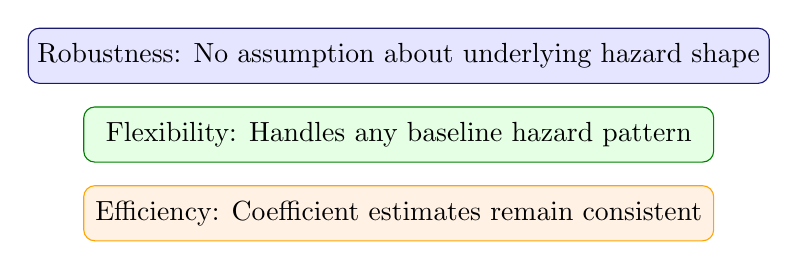
\begin{tikzpicture}[node distance=1cm]
\tikzstyle{adv} = [rectangle, rounded corners, minimum width=8cm, minimum height=0.7cm, text centered]

\node (A1) [adv, draw=MidnightBlue, fill=blue!10] {Robustness: No assumption about underlying hazard shape};
\node (A2) [adv, below of=A1, draw=Green, fill=green!10] {Flexibility: Handles any baseline hazard pattern};
\node (A3) [adv, below of=A2, draw=Orange, fill=orange!10] {Efficiency: Coefficient estimates remain consistent};
\end{tikzpicture}
\end{center}
\end{block}
\end{frame}

\begin{frame}{Log-Linear Formulation}
Taking the natural logarithm of the Cox model linearizes the relationship:

\begin{block}{Log-Transformation}
\begin{align*}
\log h(t|X) &= \log h_0(t) + \beta_1 X_1 + \cdots + \beta_k X_k \\
            &= \log h_0(t) + \beta^T X
\end{align*}
\end{block}

\begin{block}{Interpretation of Coefficients}
The coefficient $\beta_j$ represents the change in the log-hazard associated with a one-unit increase in $X_j$:
$$\beta_j = \log\left(\frac{h(t|X_j+1)}{h(t|X_j)}\right)$$
\end{block}

\begin{center}
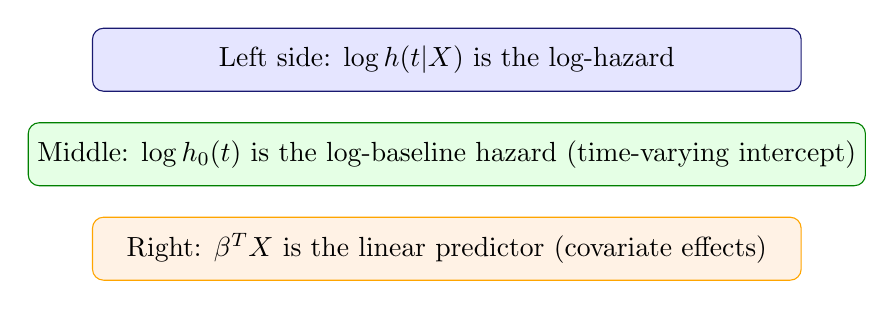
\begin{tikzpicture}[node distance=1.2cm]
\tikzstyle{interpret} = [rectangle, rounded corners, minimum width=9cm, minimum height=0.8cm, text centered]

\node (I1) [interpret, draw=MidnightBlue, fill=blue!10] {Left side: $\log h(t|X)$ is the log-hazard};
\node (I2) [interpret, below of=I1, draw=Green, fill=green!10] {Middle: $\log h_0(t)$ is the log-baseline hazard (time-varying intercept)};
\node (I3) [interpret, below of=I2, draw=Orange, fill=orange!10] {Right: $\beta^T X$ is the linear predictor (covariate effects)};
\end{tikzpicture}
\end{center}
\end{frame}

\begin{frame}{Key Feature: Proportional Hazards}
The term "proportional hazards" refers to the constant ratio of hazards:

\begin{block}{Proportionality Assumption}
For any two individuals with covariates $X_A$ and $X_B$:
$$\frac{h(t|X_A)}{h(t|X_B)} = \frac{h_0(t) \exp(\beta^T X_A)}{h_0(t) \exp(\beta^T X_B)} = \exp(\beta^T (X_A - X_B))$$
This ratio is constant for all time $t$.
\end{block}

\begin{center}
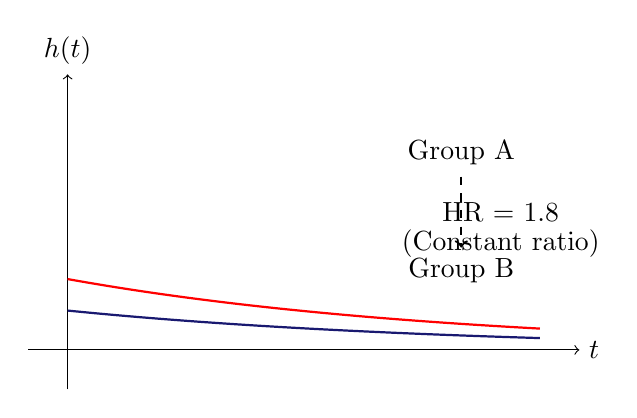
\begin{tikzpicture}[domain=0:6, smooth, samples=100]
\draw[->] (-0.5,0) -- (6.5,0) node[right] {$t$};
\draw[->] (0,-0.5) -- (0,3.5) node[above] {$h(t)$};

\draw[thick, MidnightBlue] plot (\x, {0.5*exp(-0.2*\x)});
\draw[thick, red] plot (\x, {0.5*exp(-0.2*\x)*1.8});

\node at (5,2.5) {Group A};
\node at (5,1) {Group B};
\draw[->, thick, dashed] (5,2.2) -- (5,1.3);
\node at (5.5,1.75) {HR = 1.8};
\node at (5.5,1.35) {(Constant ratio)};
\end{tikzpicture}
\end{center}
\end{frame}

% ============================================================================
% SECTION 3: HAZARD RATIOS
% ============================================================================

\section{Hazard Ratios: Definition and Interpretation}

\subsection{Defining the Hazard Ratio}

\begin{frame}{The Hazard Ratio as a Measure of Effect}
The hazard ratio (HR) is the primary measure of association in survival analysis:

\begin{definition}[Hazard Ratio]
The hazard ratio compares the hazards of two groups:
$$\text{HR} = \frac{h(t|X_A)}{h(t|X_B)}$$
where $X_A$ and $X_B$ represent different covariate patterns.
\end{definition}

\begin{block}{Derivation from Cox Model}
\begin{align*}
\text{HR} &= \frac{h_0(t) \exp(\beta^T X_A)}{h_0(t) \exp(\beta^T X_B)} \\
          &= \exp\left(\beta^T (X_A - X_B)\right)
\end{align*}
The baseline hazard cancels out, leaving only the covariate effects.
\end{block}
\end{frame}

\begin{frame}{Hazard Ratio for a Single Covariate}
For a binary exposure $X$ (0 = unexposed, 1 = exposed):

\begin{block}{Model}
$$h(t|X) = h_0(t) \exp(\beta X)$$
\end{block}

\begin{block}{Hazard Ratio Calculation}
\begin{align*}
\text{HR} &= \frac{h(t|X=1)}{h(t|X=0)} \\
          &= \frac{h_0(t) \exp(\beta \cdot 1)}{h_0(t) \exp(\beta \cdot 0)} \\
          &= \exp(\beta)
\end{align*}
\end{block}

\begin{block}{Key Result}
$$\text{HR} = \exp(\beta)$$
The exponentiated coefficient directly gives the hazard ratio.
\end{block}
\end{frame}

\begin{frame}{Interpretation of Hazard Ratios}
\begin{center}
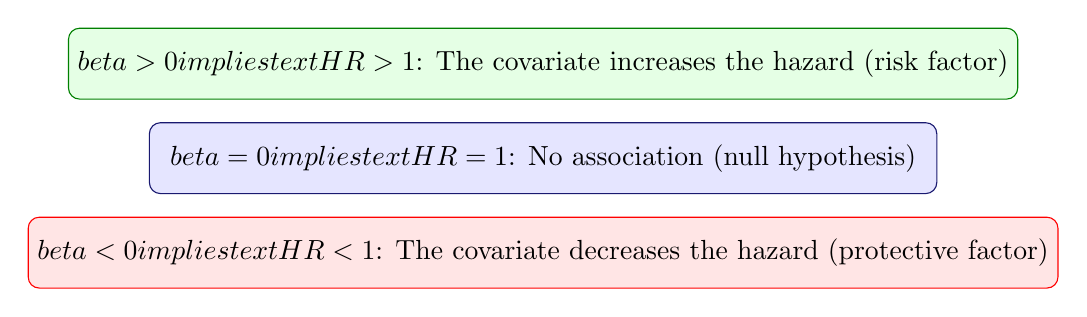
\begin{tikzpicture}[node distance=1.2cm]
\tikzstyle{interpretation} = [rectangle, rounded corners, minimum width=10cm, minimum height=0.9cm, text centered]

\node (I1) [interpretation, draw=Green, fill=green!10] {$\\beta > 0 \\implies \\text{HR} > 1$: The covariate increases the hazard (risk factor)};
\node (I2) [interpretation, below of=I1, draw=MidnightBlue, fill=blue!10] {$\\beta = 0 \\implies \\text{HR} = 1$: No association (null hypothesis)};
\node (I3) [interpretation, below of=I2, draw=Red, fill=red!10] {$\\beta < 0 \\implies \\text{HR} < 1$: The covariate decreases the hazard (protective factor)};
\end{tikzpicture}
\end{center}
\end{frame}

\begin{frame}{Numerical Interpretation Examples}
\begin{center}
\begin{tabular}{cccc}
\toprule
$\beta$ & HR = $\exp(\beta)$ & Interpretation & 95\% CI for HR \\
\midrule
0 & 1.00 & No effect & (0.82, 1.22) \\
0.10 & 1.11 & 11\% increased hazard & (0.91, 1.35) \\
0.20 & 1.22 & 22\% increased hazard & (1.00, 1.49) \\
0.50 & 1.65 & 65\% increased hazard & (1.35, 2.02) \\
1.00 & 2.72 & 172\% increased hazard & (2.23, 3.32) \\
-0.10 & 0.90 & 10\% decreased hazard & (0.74, 1.10) \\
-0.20 & 0.82 & 18\% decreased hazard & (0.67, 1.00) \\
-0.50 & 0.61 & 39\% decreased hazard & (0.50, 0.74) \\
-1.00 & 0.37 & 63\% decreased hazard & (0.30, 0.45) \\
\bottomrule
\end{tabular}
\end{center}
\end{frame}

\begin{frame}{Continuous Covariates: Unit Changes}
For a continuous predictor, the HR represents the hazard ratio per unit increase:

\begin{block}{Model}
$$h(t|X) = h_0(t) \exp(\beta X)$$
where $X$ is a continuous variable (e.g., age, blood pressure).
\end{block}

\begin{block}{Interpretation}
For a one-unit increase in $X$:
$$\text{HR} = \exp(\beta)$$

For a $c$-unit increase:
$$\text{HR}_{c} = \exp(c \cdot \beta)$$
\end{block}

\begin{block}{Example: Age and Cardiovascular Disease}
If $\beta_{\text{age}} = 0.08$ (per year):
\begin{itemize}
\item Per 1 year: $\text{HR} = \exp(0.08) = 1.083$ (8.3\% increased hazard)
\item Per 10 years: $\text{HR} = \exp(0.80) = 2.23$ (123\% increased hazard)
\end{itemize}
\end{block}
\end{frame}

% ============================================================================
% SECTION 4: ESTIMATION AND CENSORING
% ============================================================================

\section{Estimation and the Role of Censoring}

\subsection{Partial Likelihood}

\begin{frame}{Estimating Cox Model Coefficients}
Unlike parametric models, the Cox model uses partial likelihood:

\begin{block}{Cox (1972) Insight}
Since $h_0(t)$ cancels out in the hazard ratio, we can estimate $\beta$ without estimating $h_0(t)$.
\end{block}

\begin{block}{Partial Likelihood Principle}
At each event time $t_j$, the probability that individual $i$ (who experienced the event) had the event, given that one event occurred in the risk set $R(t_j)$, is:
$$L(\beta) = \prod_{j=1}^{D} \frac{\exp(\beta^T X_i)}{\sum_{l \in R(t_j)} \exp(\beta^T X_l)}$$
where $D$ is the number of distinct event times.
\end{block}
\end{frame}

\begin{frame}{The Risk Set Concept}
The risk set $R(t_j)$ contains all individuals still under observation just before time $t_j$:

\begin{center}
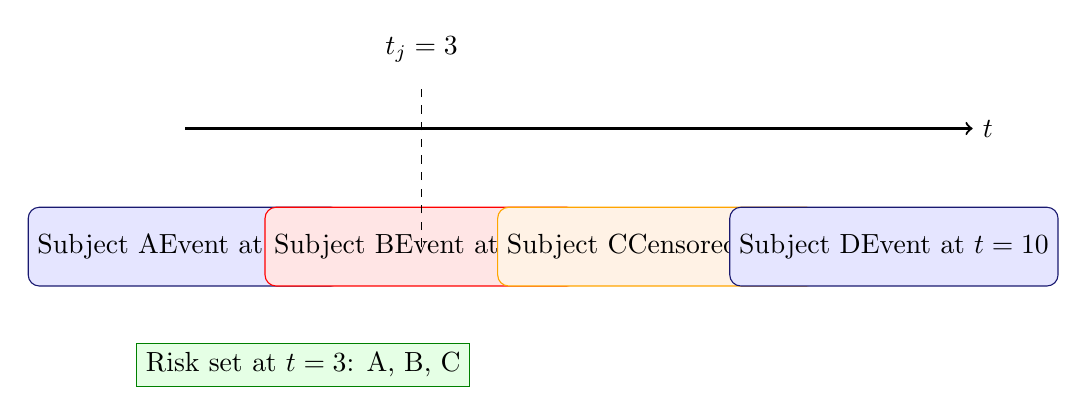
\begin{tikzpicture}[node distance=1.5cm]
\tikzstyle{block} = [rectangle, rounded corners, minimum width=3cm, minimum height=1cm, text centered, draw=MidnightBlue, fill=blue!10]
\tikzstyle{event} = [rectangle, rounded corners, minimum width=1.5cm, minimum height=1cm, text centered, draw=Red, fill=red!10]
\tikzstyle{censor} = [rectangle, rounded corners, minimum width=1.5cm, minimum height=1cm, text centered, draw=Orange, fill=orange!10]

\node (time0) at (0,0) [block] {Subject A\\Event at $t=5$};
\node (time1) at (3,0) [event] {Subject B\\Event at $t=3$};
\node (time2) at (6,0) [censor] {Subject C\\Censored $t=7$};
\node (time3) at (9,0) [block] {Subject D\\Event at $t=10$};

\node at (1.5,-1.5) [rectangle, draw=Green, fill=green!10, minimum width=4cm] {Risk set at $t=3$: A, B, C};

\draw[->, thick] (0,1.5) -- (10,1.5) node[right] {$t$};

\node at (3,2.5) {$t_j = 3$};
\draw[dashed] (3,0) -- (3,2);
\end{tikzpicture}
\end{center}

\begin{block}{Risk Set Composition}
At time $t_j$:
\begin{itemize}
\item Include all subjects who have not yet experienced the event
\item Include all uncensored subjects (censored subjects leave the risk set at their censoring time)
\end{itemize}
\end{block}
\end{frame}

\begin{frame}{Incorporating Censoring in Partial Likelihood}
Censored observations contribute to the likelihood through their presence in risk sets:

\begin{block}{Censoring Mechanism}
\begin{center}
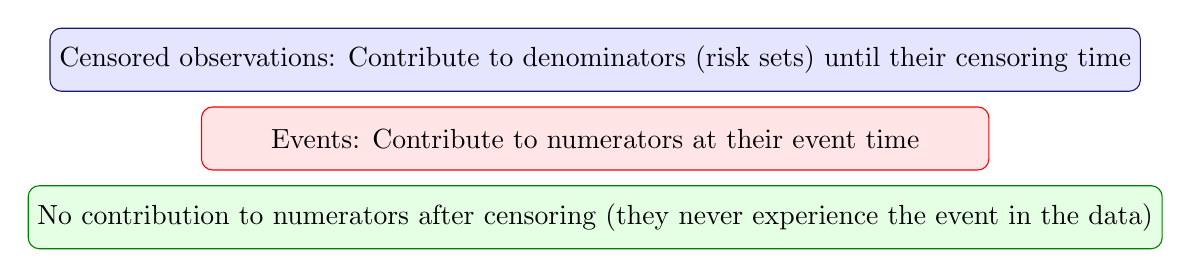
\begin{tikzpicture}[node distance=1cm]
\tikzstyle{contribution} = [rectangle, rounded corners, minimum width=10cm, minimum height=0.8cm, text centered]

\node (C1) [contribution, draw=MidnightBlue, fill=blue!10] {Censored observations: Contribute to denominators (risk sets) until their censoring time};
\node (C2) [contribution, below of=C1, draw=Red, fill=red!10] {Events: Contribute to numerators at their event time};
\node (C3) [contribution, below of=C2, draw=Green, fill=green!10] {No contribution to numerators after censoring (they never experience the event in the data)};
\end{tikzpicture}
\end{center}
\end{block}

\begin{block}{Assumption}
This approach assumes non-informative censoring: the probability of being censored does not depend on the unobserved event time.
\end{block}
\end{frame}

\begin{frame}{Variance Estimation and Inference}
After maximizing the partial likelihood:

\begin{block}{Observed Information Matrix}
The variance-covariance matrix of $\hat{\beta}$ is estimated from the observed information:
$$\widehat{\text{Cov}}(\hat{\beta}) = I(\hat{\beta})^{-1}$$
where $I(\beta)$ is the Fisher information matrix.
\end{block}

\begin{block}{Wald Tests for Coefficients}
For testing $H_0: \beta_j = 0$:
$$z = \frac{\hat{\beta}_j}{\text{SE}(\hat{\beta}_j)} \sim \mathcal{N}(0,1)$$
95\% CI for $\beta_j$: $\hat{\beta}_j \pm 1.96 \cdot \text{SE}(\hat{\beta}_j)$
\end{block}

\begin{block}{Confidence Intervals for HR}
95\% CI for $\text{HR}_j$: $\left(\exp(\hat{\beta}_j - 1.96 \cdot \text{SE}), \exp(\hat{\beta}_j + 1.96 \cdot \text{SE})\right)$
\end{block}
\end{frame}

% ============================================================================
% SECTION 5: PROPORTIONAL HAZARDS ASSUMPTION
% ============================================================================

\section{The Proportional Hazards Assumption}

\subsection{Understanding and Checking the Assumption}

\begin{frame}{The Proportional Hazards Assumption}
The proportional hazards (PH) assumption is the cornerstone of the Cox model:

\begin{alertblock}{The Assumption}
The hazard ratio comparing any two covariate patterns is constant over time:
$$\frac{h(t|X_A)}{h(t|X_B)} = \text{constant for all } t$$
\end{alertblock}

\begin{block}{Implications of PH}
\begin{columns}
\begin{column}{0.5\textwidth}
\begin{block}{Mathematical}
The effect of each covariate on the hazard is multiplicative and time-independent.
\end{block}
\end{column}
\begin{column}{0.5\textwidth}
\begin{block}{Graphical}
Hazard curves for different groups should be parallel on the log-hazard scale.
\end{block}
\end{column}
\end{columns}
\end{block}
\end{frame}

\begin{frame}{Violations of Proportional Hazards}
When the PH assumption is violated, the interpretation of the HR becomes problematic:

\begin{center}
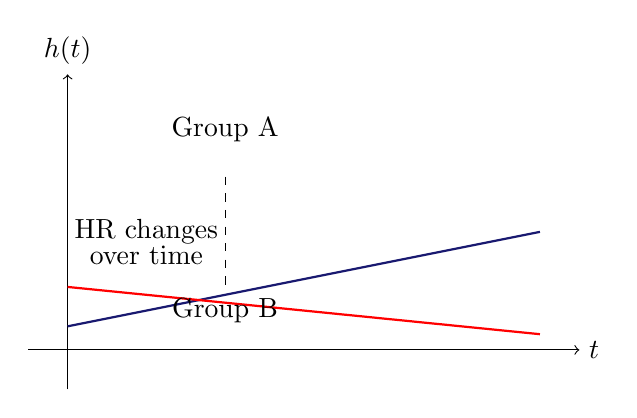
\begin{tikzpicture}[domain=0:6, smooth, samples=100]
\draw[->] (-0.5,0) -- (6.5,0) node[right] {$t$};
\draw[->] (0,-0.5) -- (0,3.5) node[above] {$h(t)$};

\draw[thick, MidnightBlue] plot (\x, {0.3 + 0.2*\x});
\draw[thick, red] plot (\x, {0.8 - 0.1*\x});

\node at (2,2.8) {Group A};
\node at (2,0.5) {Group B};
\draw[dashed] (2,2.2) -- (2,0.8);
\node at (1,1.5) {HR changes};
\node at (1,1.2) {over time};
\end{tikzpicture}
\end{center}

\begin{block}{Types of Violations}
\begin{center}
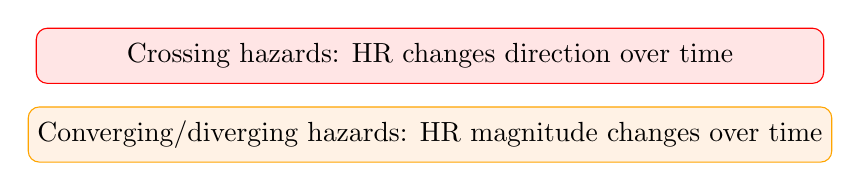
\begin{tikzpicture}[node distance=1cm]
\tikzstyle{violation} = [rectangle, rounded corners, minimum width=10cm, minimum height=0.7cm, text centered]

\node (V1) [violation, draw=Red, fill=red!10] {Crossing hazards: HR changes direction over time};
\node (V2) [violation, below of=V1, draw=Orange, fill=orange!10] {Converging/diverging hazards: HR magnitude changes over time};
\end{tikzpicture}
\end{center}
\end{block}
\end{frame}

\begin{frame}{Methods for Checking the PH Assumption}
Several diagnostic methods assess the PH assumption:

\begin{block}{Graphical Methods}
\begin{itemize}
\item \textbf{Log-minus-log plots}: Plot $\log(-\log S(t))$ for different groups; parallel lines suggest PH holds
\item \textbf{Kaplan-Meier curves}: Visual inspection of survival curves crossing
\end{itemize}
\end{block}

\begin{block}{Statistical Tests}
\begin{itemize}
\item \textbf{Schoenfeld residuals}: Test for correlation between residuals and time
\begin{equation*}
\text{Test statistic} = \sum_{j=1}^{D} (t_j - \bar{t}) r_j
\end{equation*}
where $r_j$ are the scaled Schoenfeld residuals
\item \textbf{Grambsch-Therneau test}: Formal test for non-zero slope
\end{itemize}
\end{block}
\end{frame}

\begin{frame}{Addressing Non-Proportional Hazards}
When PH is violated, several approaches exist:

\begin{center}
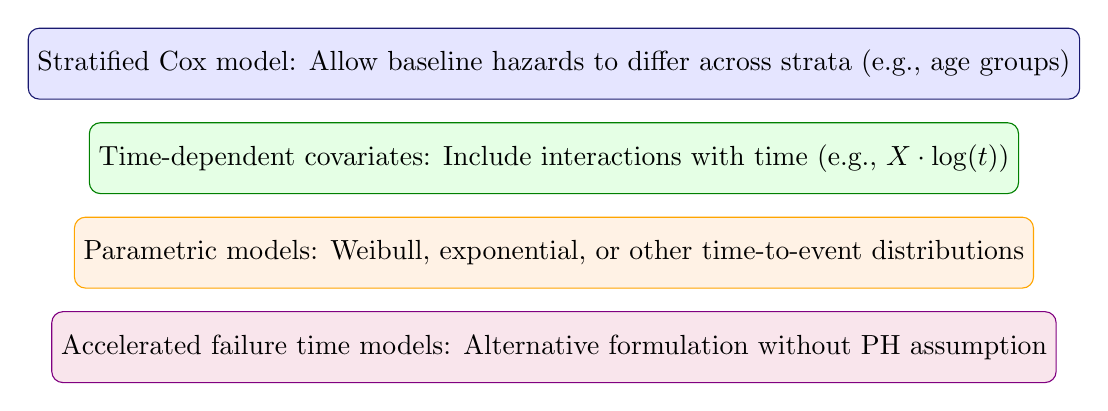
\begin{tikzpicture}[node distance=1.2cm]
\tikzstyle{solution} = [rectangle, rounded corners, minimum width=10cm, minimum height=0.9cm, text centered]

\node (S1) [solution, draw=MidnightBlue, fill=blue!10] {Stratified Cox model: Allow baseline hazards to differ across strata (e.g., age groups)};
\node (S2) [solution, below of=S1, draw=Green, fill=green!10] {Time-dependent covariates: Include interactions with time (e.g., $X \cdot \log(t)$)};
\node (S3) [solution, below of=S2, draw=Orange, fill=orange!10] {Parametric models: Weibull, exponential, or other time-to-event distributions};
\node (S4) [solution, below of=S3, draw=Purple, fill=purple!10] {Accelerated failure time models: Alternative formulation without PH assumption};
\end{tikzpicture}
\end{center}
\end{frame}

% ============================================================================
% SECTION 6: PUBLIC HEALTH INTERPRETATION
% ============================================================================

\section{Hazard Ratios in Public Health Context}

\begin{frame}{Interpreting Hazard Ratios in Epidemiology}
The hazard ratio provides a measure of relative risk over time:

\begin{block}{Definition in Context}
The hazard ratio represents the instantaneous relative risk of the event at any point in time, comparing two exposure groups.
\end{block}

\begin{block}{Example: Smoking and Lung Cancer}
In a cohort study following 10,000 participants for 20 years:
\begin{center}
\begin{tabular}{lccc}
\toprule
Exposure & Events & Person-Years & Hazard Rate \\
\midrule
Smokers & 320 & 80,000 & 0.0040 \\
Non-smokers & 80 & 120,000 & 0.0007 \\
\bottomrule
\end{tabular}
\end{center}
$$\text{HR} = \frac{0.0040}{0.0007} = 5.7$$
Interpretation: At any given time, smokers have 5.7 times the hazard of lung cancer death compared to non-smokers.
\end{block}
\end{frame}

\begin{frame}{Hazard Ratio vs. Risk Ratio vs. Odds Ratio}
Understanding the distinctions:

\begin{center}
\begin{tabular}{p{3cm}p{4cm}p{4cm}}
\toprule
Measure & Definition & Interpretation \\
\midrule
\textbf{Risk Ratio (RR)} & $P(\text{Event}|X=1) / P(\text{Event}|X=0)$ & Cumulative risk over study period \\
\midrule
\textbf{Odds Ratio} & Odds(Event$|$X=1) / Odds(Event$|$X=0) & Cross-sectional or case-control \\
\midrule
\textbf{Hazard Ratio} & $h(t|X=1) / h(t|X=0)$ & Instantaneous rate at any time $t$ \\
\bottomrule
\end{tabular}
\end{center}

\begin{block}{Key Distinction}
The HR compares instantaneous rates at any point in time, while RR and OR compare cumulative measures. When the event is rare, all three approximate each other.
\end{block}
\end{frame}

\begin{frame}{Public Health Applications of Cox Models}
Cox proportional hazards models are widely used in public health research:

\begin{center}
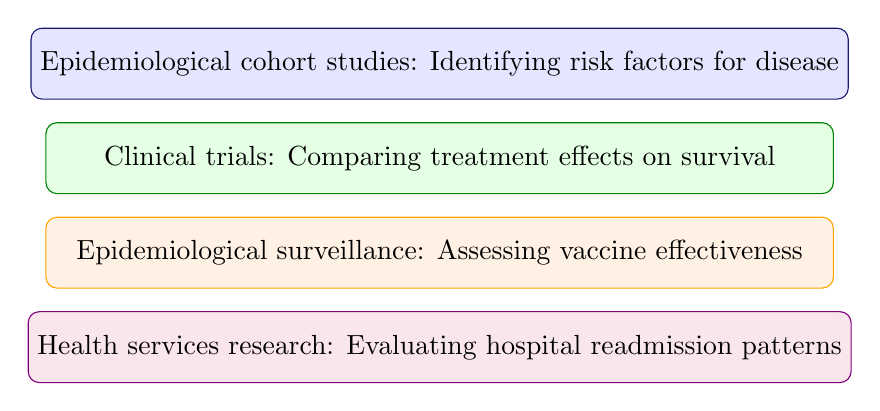
\begin{tikzpicture}[node distance=1.2cm]
\tikzstyle{application} = [rectangle, rounded corners, minimum width=10cm, minimum height=0.9cm, text centered]

\node (A1) [application, draw=MidnightBlue, fill=blue!10] {Epidemiological cohort studies: Identifying risk factors for disease};
\node (A2) [application, below of=A1, draw=Green, fill=green!10] {Clinical trials: Comparing treatment effects on survival};
\node (A3) [application, below of=A2, draw=Orange, fill=orange!10] {Epidemiological surveillance: Assessing vaccine effectiveness};
\node (A4) [application, below of=A3, draw=Purple, fill=purple!10] {Health services research: Evaluating hospital readmission patterns};
\end{tikzpicture}
\end{center}
\end{frame}

\begin{frame}{Example: COVID-19 Vaccine Effectiveness}
Real-world application of Cox models in pandemic research:

\begin{block}{Study Design}
Retrospective cohort study of vaccine effectiveness against hospitalization.
\end{block}

\begin{block}{Model}
$$h(t|\text{vaccine}) = h_0(t) \exp(\beta \cdot \text{vaccine})$$
\end{block}

\begin{block}{Results}
\begin{center}
\begin{tabular}{lcc}
\toprule
Vaccine Status & HR & 95\% CI \\
\midrule
Unvaccinated (Reference) & 1.00 & - \\
Two doses & 0.15 & (0.10, 0.22) \\
Booster dose & 0.05 & (0.03, 0.08) \\
\bottomrule
\end{tabular}
\end{center}
\end{block}

\begin{block}{Interpretation}
Booster vaccination reduced the hazard of COVID-19 hospitalization by 95\% compared to unvaccinated individuals.
\end{block}
\end{frame}

\begin{frame}{Statistical vs. Clinical Significance}
Assessing the practical importance of hazard ratios:

\begin{block}{Statistical Significance}
Based on whether the 95\% CI for HR excludes 1.0:
\begin{itemize}
\item $p < 0.05$ suggests the association is unlikely due to chance
\end{itemize}
\end{block}

\begin{block}{Clinical/Public Health Significance}
Consider the magnitude of effect:
\begin{center}
\begin{tabular}{ll}
\toprule
HR Range & Interpretation \\
\midrule
0.90 - 1.10 & Negligible effect \\
0.75 - 0.90 or 1.10 - 1.33 & Small effect \\
0.50 - 0.75 or 1.33 - 2.00 & Moderate effect \\
< 0.50 or > 2.00 & Large effect \\
\bottomrule
\end{tabular}
\end{center}
\end{block}
\end{frame}

% ============================================================================
% SECTION 7: CONCLUSION
% ============================================================================

\section{Conclusion}

\begin{frame}{Summary: Key Concepts}
\begin{center}
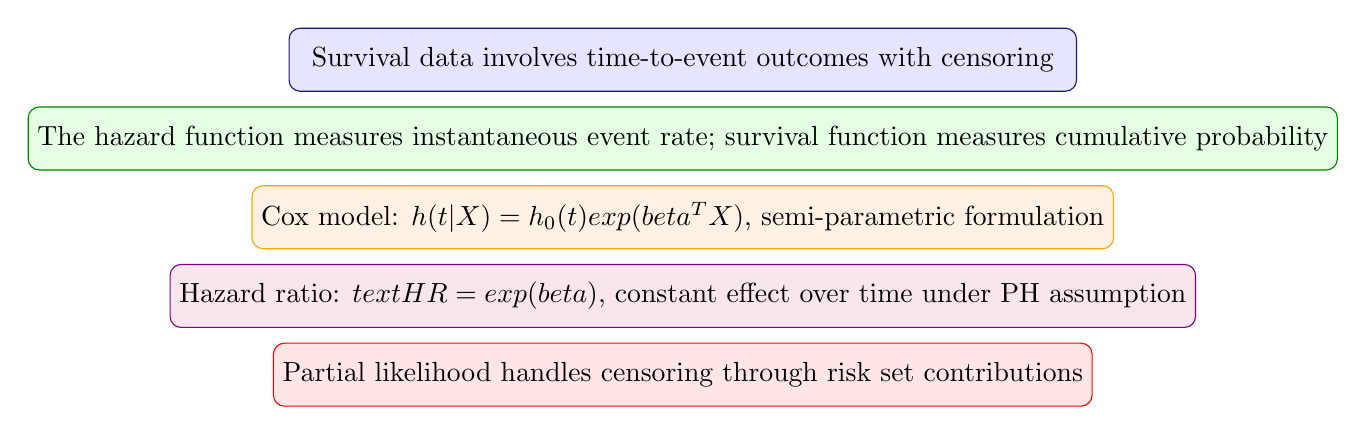
\begin{tikzpicture}[node distance=1cm]
\tikzstyle{summary} = [rectangle, rounded corners, minimum width=10cm, minimum height=0.8cm, text centered]

\node (S1) [summary, draw=MidnightBlue, fill=blue!10] {Survival data involves time-to-event outcomes with censoring};
\node (S2) [summary, below of=S1, draw=Green, fill=green!10] {The hazard function measures instantaneous event rate; survival function measures cumulative probability};
\node (S3) [summary, below of=S2, draw=Orange, fill=orange!10] {Cox model: $h(t|X) = h_0(t)\\exp(\\beta^T X)$, semi-parametric formulation};
\node (S4) [summary, below of=S3, draw=Purple, fill=purple!10] {Hazard ratio: $\\text{HR} = \\exp(\\beta)$, constant effect over time under PH assumption};
\node (S5) [summary, below of=S4, draw=Red, fill=red!10] {Partial likelihood handles censoring through risk set contributions};
\end{tikzpicture}
\end{center}
\end{frame}

\begin{frame}{Key Equations Summary}
\begin{center}
\begin{small}
\begin{align*}
\textbf{Hazard Function:} \quad & h(t) = \\lim_{\\Delta t \\to 0} \\frac{P(t \\le T < t + \\Delta t | T \\ge t)}{\\Delta t} \\\\
\textbf{Survival Function:} \quad & S(t) = P(T > t) \\\\
\textbf{Cox Model:} \quad & h(t|X) = h_0(t) \\exp(\\beta_1 X_1 + \\cdots + \\beta_k X_k) \\\\
\textbf{Hazard Ratio:} \quad & \\text{HR} = \\exp(\\beta_j) \\quad \\text{(for 1-unit change in } X_j\\text{)} \\\\
\textbf{Data Representation:} \quad & \\text{Observed time } t_i = \\min(T_i, C_i), \\quad \\delta_i = I(T_i \\le C_i)
\end{align*}
\end{small}
\end{center}
\end{frame}

\begin{frame}{Final Takeaways for Public Health Practice}
\begin{columns}
\begin{column}{0.5\textwidth}
\begin{block}{Strengths of Cox Model}
\begin{itemize}
\item Handles censored data naturally
\item Semi-parametric form is flexible
\item Provides intuitive HR measures
\end{itemize}
\end{block}
\end{column}
\begin{column}{0.5\textwidth}
\begin{block}{Key Considerations}
\begin{itemize}
\item Verify proportional hazards assumption
\item Consider time-dependent effects if needed
\end{itemize}
\end{block}
\end{column}
\end{columns}

\begin{center}
\textbf{"The Cox proportional hazards model remains the cornerstone of survival analysis in epidemiology, providing a powerful framework for quantifying the effects of risk factors on time-to-event outcomes."}
\end{center}
\end{frame}

\begin{frame}{References}
\begin{small}
\begin{itemize}
\item Cox, D.R. (1972). Regression Models and Life-Tables (with discussion). Journal of the Royal Statistical Society, Series B, 34(2), 187-220.
\item Kleinbaum, D.G. and Klein, M. (2012). Survival Analysis: A Self-Learning Text (3rd ed.). Springer.
\item Therneau, T.M. and Grambsch, P.M. (2000). Modeling Survival Data: Extending the Cox Model. Springer.
\item Hosmer, D.W., Lemeshow, S., and May, S. (2008). Applied Survival Analysis: Regression Modeling of Time to Event Data (2nd ed.). Wiley.
\end{itemize}
\end{small}
\end{frame}

\end{document}
